\subsection*{Case Study}
Our case-study is the model built to describe an Information Management System for the \textit{MWK (Manages With Knowledge)} project. This modeling was developed in the context of the Software Systems Development course. 

\begin{figure}[!htbp]
\begin{center}
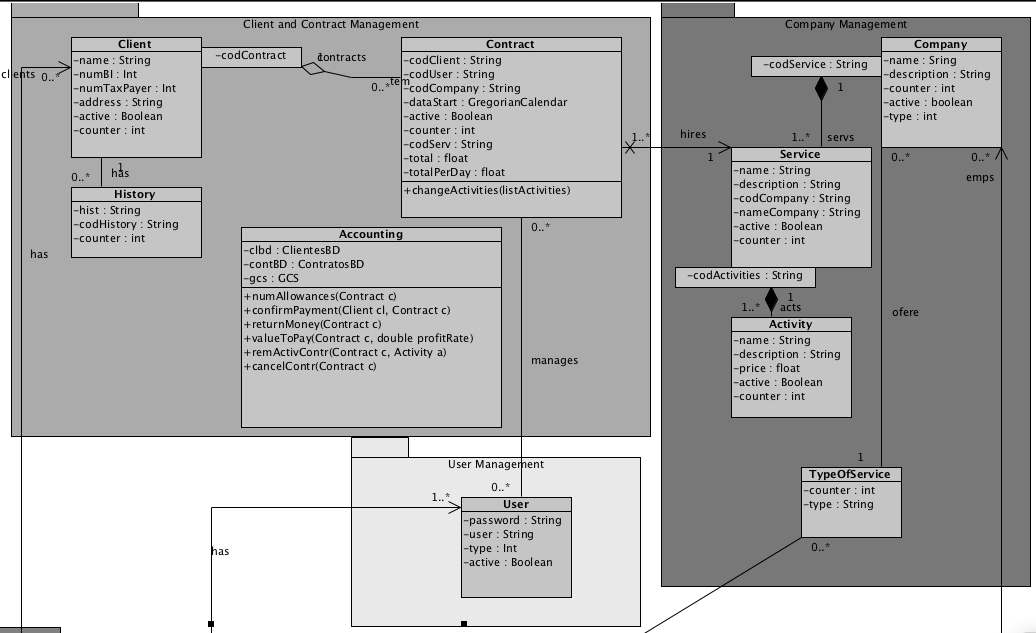
\includegraphics[scale=0.345]{images/classbw.png}
\caption{Excerpt of a Class diagram}\label{fig:class}
\end{center}
\end{figure} 

In order to meet its clients needs \emph{MKW} is a company that has a wide range of suppliers subcontracted to be responsible for services execution.
Multiple suppliers can supply the same service and each service can be delivered in different ways.
Each service can then be composed of multiple activities. As an example, there could be a service called \textit{Shirts until 10 Kg} and inside this service there could be activities such as \textit{wash, iron, sewing buttons, etc}.
Each activity of a given service as a stipulated price, and can be hired by a client.
%The goal of the project was to model and implement a management software for this task.

\begin{figure}[!htbp]
\begin{center}
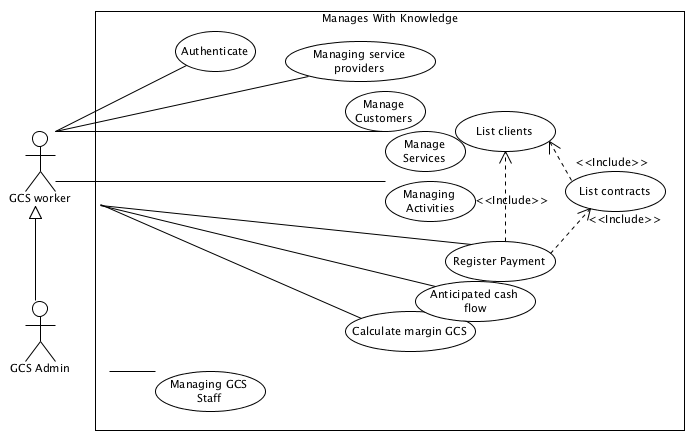
\includegraphics[width=0.9\textwidth]{images/usecase.png}
\caption{The general Use Case model}\label{fig:usecase}
\end{center}
\end{figure} 

As an example of the \uml\ diagrams used to model this task, we can see in Figure \ref{fig:usecase} an image of a general Use Case diagram and, in Figure \ref{fig:class}, an excerpt of a class diagram.

Adding to Use Case and Class diagrams, the modelation is composed of Sequence and State Machine diagrams.
